\documentclass[UTF8]{ctexart}

\usepackage[backend=bibtex]{biblatex}
\usepackage{mathtools}
\usepackage[CJKbookmarks=true,colorlinks,linkcolor=blue,anchorcolor=blue,citecolor=green]{hyperref}
\usepackage{color}
\usepackage{graphicx}
\usepackage{enumerate}
\usepackage{titlesec}
\usepackage{titletoc}
\usepackage{bm}

\newcommand{\HRule}{\rule{\linewidth}{0.5mm}}
\newcommand{\myFunc}{}
\newenvironment{myquote}
  {\begin{quote}\kaishu\zihao{-5}}
  {\end{quote}}

\titlecontents{section}
              [0em]
              {\bf \small}%
              {\contentslabel{2.5em}}%
              {}%
              {\titlerule*[0.5pc]{$\cdot$}\contentspage}%

\begin{document}
\begin{titlepage}
\begin{center}

\includegraphics[width=\textwidth]{UESTC-Logo}\\[2cm]
\textsc{\LARGE 计算机学院~$\bullet$~人工智能应用与挑战课程~}\\[1.5cm]
\HRule \\[0.4cm]
{ \huge \bfseries Northeastern SMILE Lab - Recognizing Faces in the Wild项目中期报告\\[0.4cm] }

\HRule \\[1.5cm]
\noindent
\emph{组名}:\quad
\quad {\bf Honkai StarRail}\\
\emph{作者}:\quad
\quad {\bf 刘*}\footnotemark
\quad {\bf 赵**}\footnotemark
\quad {\bf 武**}\footnotemark\\
\emph{指导老师}:\quad
\quad {\bf 文泉}
\end{center}
\footnotetext[1]{电子科技大学计算机科学与工程学院数字媒体技术专业,学号:2022**}
\footnotetext[2]{电子科技大学计算机科学与工程学院数字媒体技术专业,学号:2022**}
\footnotetext[3]{电子科技大学计算机科学与工程学院计算机科学与技术专业,学号:2022**}
\end{titlepage}

\tableofcontents
\newpage

\section{前言}
本篇报告为计算机学院~$\bullet$~人工智能应用与挑战课程~,Honkai StarRail小组的项目中期报告,小组选题为“Northeastern SMILE Lab - Recognizing Faces in the Wild”,(详见网址:\href{https://www.kaggle.com/competitions/recognizing-faces-in-the-wild}{小组选题})。

本篇报告包括项目概况介绍、项目中期进展情况、中期进展后拟改进措施三部分。

\section{题目概况}
\subsection{竞赛概况}
我们的选题名为“Northeastern SMILE Lab - Recognizing Faces in the Wild”:基于人脸识别的血缘关系鉴定模型(图:$\left(\ref{fig:competition}\right)$)。本次竞赛的主办方为东北大学的微笑实验室\footnote{Northeastern SMILE Lab},该实验室的研究课题有"Effects of Speech Modification Strategies on Vowel Acoustics for Adolescents with Cerebral Palsy"、"Development of Auditory-Perceptual Speech Features in Preschoolers with Typical Development"、"Innovations in the Evaluation and Management of Pediatric Dysarthria"等\footnote{详见东北大学微笑实验室网址:https://smilelab.sites.northeastern.edu}。

\begin{figure}[!ht]
  \centering
  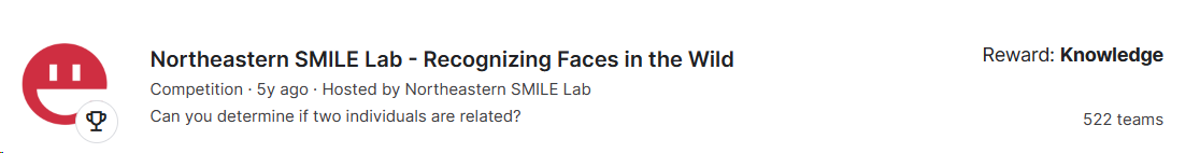
\includegraphics[width=1\textwidth]{competition.png}
  \caption{竞赛题目}
  \label{fig:competition}
\end{figure}

该竞赛的开始时间为2019年5月14日,结束时间为2019年8月9日,竞赛类型为playground。虽然本次竞赛没有实物奖励,但由于该竞赛的题目较有意思,吸引了522支队伍、573位选手参加该竞赛。

\subsection{竞赛内容}
在该竞赛中,题目要求参赛者训练一个模型图像识别模型,该模型能仅通过图像鉴定两人是否有血缘关系。由于用于亲属识别任务的现有图像数据库规模不足以捕捉和反映世界各地家庭的真实数据分布,并且许多隐藏因素会影响家族面部关系,因此需要比计算机视觉算法更有区分度的模型,这也是本竞赛被提出的原因。

由于该竞赛考察的是参赛者模型的识别正确率,故该竞赛的评分标准为\[Score=\frac{N}{M}\],其中N为正确识别血缘关系的测试集数量,M为测试集总数。排行榜也是依据参赛者模型的识别正确率进行排名。

\subsection{竞赛意义}
当今社会,血缘关系鉴定有着多方面、多维度的社会意义:
\begin{itemize}
  \item 当家庭中存在怀疑亲子关系的情况时,血缘关系鉴定有助于维护家庭的稳定与和谐。
  \item 当在法律上出现亲子权纠纷、抚养权争议等问题时,血缘关系鉴定有利于保障当事人的合法权益。
  \item 当对某些人的身份存疑时,如失踪人员寻亲、被拐卖儿童寻亲等,血缘关系鉴定可帮助确认个人身份与亲属关系。
  \item 在医学上可以帮助研究家族遗传病的遗传模式、基因突变的传播等,辅助控制家族遗传病的产生。
\end{itemize}

而现如今最常用的血缘鉴定方式为依据遗传学的基本原理,采用现代化的DNA分型检测技术来综合评判争议个体之间是否存在亲生、隔代或其他血缘关系\footnote{详见https://baike.120ask.com/art/50356}。这种血缘关系鉴定需提取被鉴定者的DNA样本,并通过PCR扩增、后PCR反应、毛细管测序仪检测等步骤完成血缘鉴定,鉴定过程较为繁琐。若能开发出一套基于被鉴定者的外貌特征而实现的亲子鉴定系统,则将大大提高血缘鉴定的效率,减少血缘鉴定的成本。

\subsection{数据规模}
\subsubsection{数据集}
官方给出的测试数据共包含12个文件(详见图$\left(\ref{fig:training data}\right)$),

\begin{figure}[!ht]
  \centering
  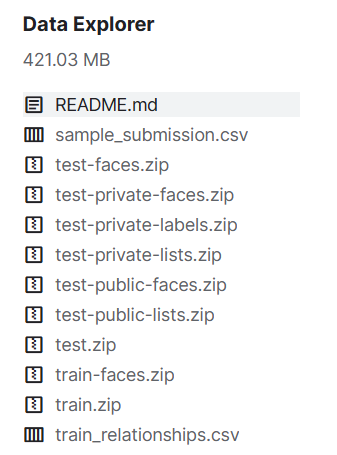
\includegraphics[width=0.5\textwidth]{training data.jpg}
  \caption{测试文件}
  \label{fig:training data}
\end{figure}
其中较为重要的分别是:
\begin{itemize}
  \item train-faces.zip,训练集被分为家庭(F0123),然后是个体(MIDx)。同一MIDx文件夹中的图像属于同一个人。同一个F0123文件夹中的图像属于同一个家庭。
  \item train.csv,培训标签。其中需要注意的是,一个家庭中并不是每个成员都有亲属关系。例如,父母与他们的孩子有亲属关系,但彼此之间没有亲属关系。
  \item test-faces.zip,该测试集中包含未知个体的人脸图像。
  \item sample\underline{\space}submission.csv,该文件为一个正确格式的示例提交文件。列\\
  img\underline{\space}pair描述了图像对,即abcd-efgh表示图像对abcd.jpg和efgh.jpg。\\
  我们的目标是预测test-faces中每对图像是否相关,其中1表示相关,0表示不相关。
\end{itemize}

以上数据文件总大小为421.03MB。

\subsubsection{提交格式} 
在该竞赛中,要求的提交格式如图$\left(\ref{fig:submission}\right)$:
\begin{figure}[!ht]
  \centering
  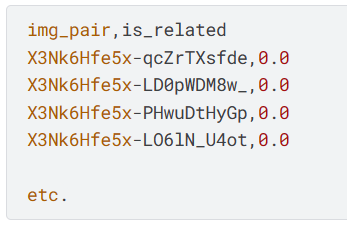
\includegraphics[width=0.5\textwidth]{submission.png}
  \caption{提交格式}
  \label{fig:submission}
\end{figure}

其中img\_pair为测试集中的图像对,图像对中有需要判断是否存在血缘关系的两张图片,is\_related则表示该图像对中的两人是否存在血缘关系,是为1,否为0。在官方给出的提交样例文件sample\underline{\space}submission.csv中,我们可以看到img\_pair与is\_related两个列向量的具体值,如图$\left(\ref{fig:sample}\right)$
\begin{figure}[!ht]
  \centering
  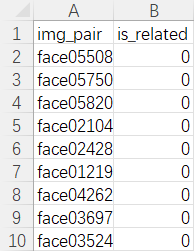
\includegraphics[width=0.5\textwidth]{sample.png}
  \caption{提交样例}
  \label{fig:sample}
\end{figure}

但在我们实际的提交过程中发现,列向量is\_related的数值可以不为0或1,若其值为img\_pair图像对具有血缘关系的可能性,这一文件也是可以被正确提交的,如图$\left(\ref{fig:mysubmission}\right)$
\begin{figure}[!ht]
  \centering
  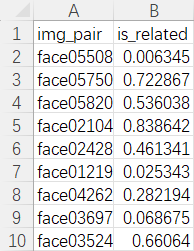
\includegraphics[width=0.5\textwidth]{mysubmission.png}
  \caption{实际提交文件}
  \label{fig:mysubmission}
\end{figure}

\subsection{现有结果}
\begin{figure}[!ht]
  \centering
  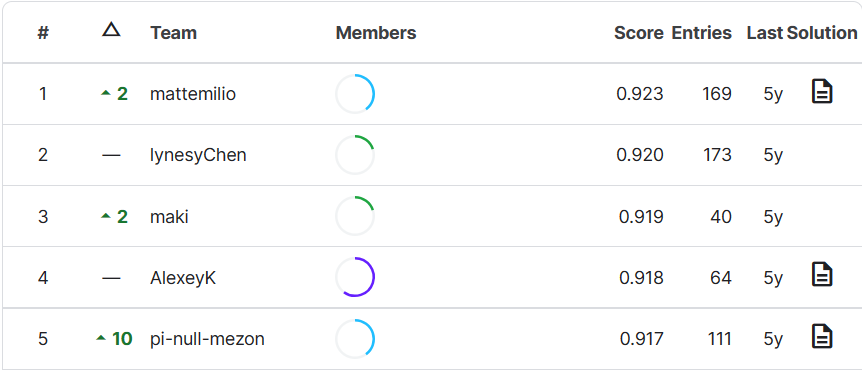
\includegraphics[width=0.7\textwidth]{leaderboard.jpg}
  \caption{排行榜1-5名}
  \label{fig:leaderboard}
\end{figure}
截至目前,共有573位参赛选手,522支参赛队伍。由于该题在五年前已完赛,故参赛选手的最终提交时间均在五年之前。

在该题目的leaderboard中(见图$\left(\ref{fig:leaderboard}\right)$),目前的世界第一为mattemilio,其得分为0.923分,前五名得分均在0.917之上,前一百名得分均在0.894之上。他们的模型识别正确率均能达到九成左右。

\section{中期进展情况}
\subsection{当前排名与结果}
本小组中期时采用的初始模型的Private Score为0.868,在Private 测试集上排名第189,Public Score为0.862,在Public测试集上排名第171。模型和数据处理方法尚未找到最优解,项目尚未成熟,因此本小组的项目仍有很大的提升空间。在中期之后,我们会考虑采用更优的数据处理方法,对模型进行不断优化。
\begin{figure}[!ht]
  \centering
  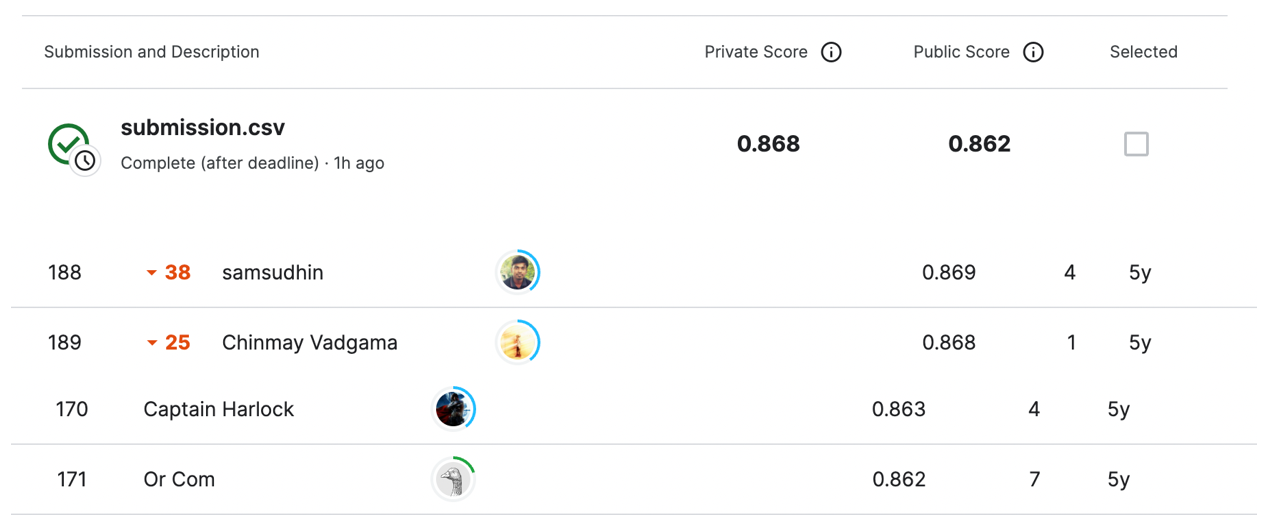
\includegraphics[width=0.7\textwidth]{score.png}
  \caption{中期排名与结果}
  \label{fig:score}
\end{figure}

\subsection{解题模型设计}
由于本项目是基于人脸识别技术的研究项目。我们选择了基于VGG-face数据集预训练的ResNet50模型作为基础模型,并借助Keras深度学习框架构建了孪生神经网络结构。在模型构建过程中,我们去除了原始模型的输出层,保留了特征提取层,并设计了自定义的输出层模型,最终采用sigmoid层作为输出。这一设计旨在通过迁移学习,充分利用已有模型在大规模数据集上学习到的特征表达能力,从而提高模型的判断准确度。我们的目标是通过人脸图像进行血缘关系的判断,因此模型的输出层需要能够有效地区分不同人脸图像之间的相似度。采用孪生神经网络结构,可以使模型在学习过程中更好地捕捉到人脸图像之间的相似性特征,从而实现更精准的血缘关系判断。
\subsubsection{模型介绍}
\begin{enumerate}
  \item ResNet50模型

  ResNet50是ResNet系列中的一个特例,它有50层深,并且采用了残差模块的结构,克服了深度神经网络训练过程中的梯度消失和梯度爆炸等问题。通过使用残差连接,ResNet50模型使得神经网络可以更深更广地构建,从而在图像识别等任务中取得了更好的性能。

  ResNet50模型的结构相对简单,主要由一系列的残差模块组成,其中包括了卷积层、批量归一化层和激活函数。整个网络的结构可以分为预处理层、卷积层、全局平均池化层和全连接层几个部分。具体结构见图$\left(\ref{fig:ResNet50}\right)$
  \begin{figure}[!ht]
    \centering
    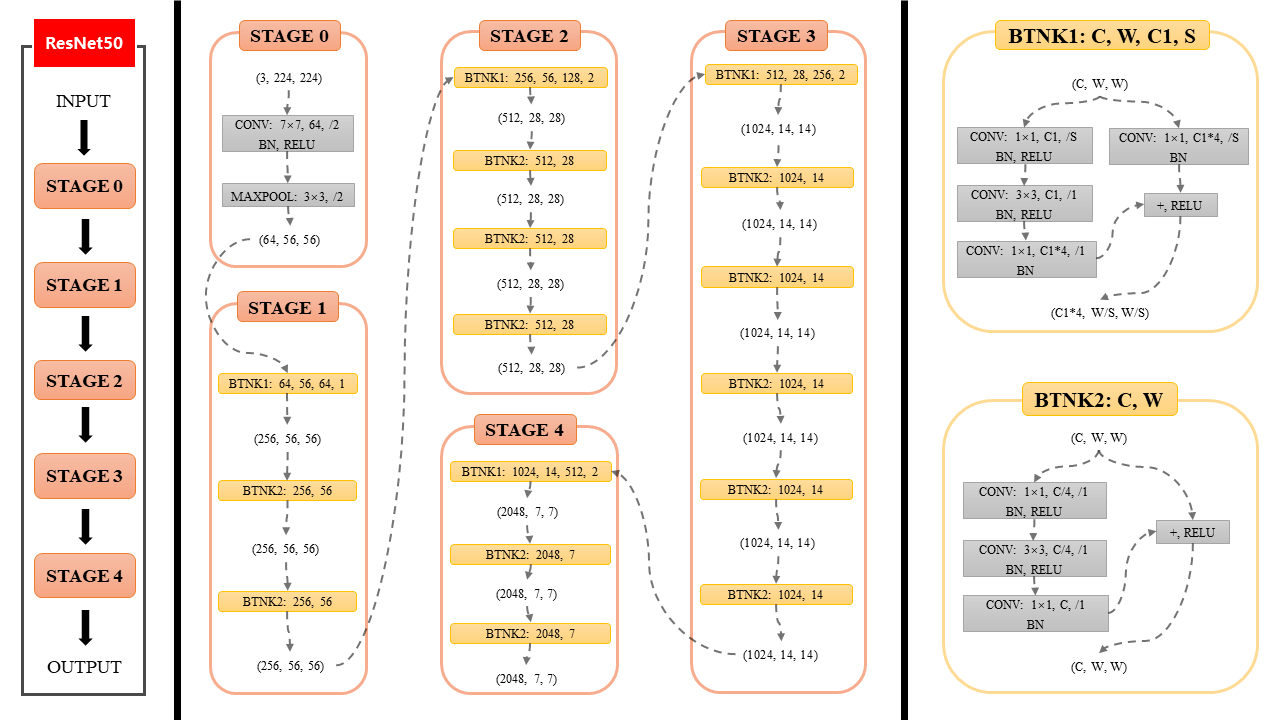
\includegraphics[width=0.7\textwidth]{ResNet50.png}
    \caption{ResNet50结构}
    \label{fig:ResNet50}
  \end{figure}
  \item 孪生神经网络
  
  孪生神经网络(Siamese Neural Network)是一种特殊的神经网络架构,最初用于解决用于度量学习(Metric Learning)的问题。孪生神经网络由两个完全相同的子网络组成,它们共享相同的权重和参数。这两个子网络被称为"孪生网络",因此得名"孪生神经网络"。

  孪生神经网络有两个输入(Input1 and Input2),将两个输入feed进入两个神经网络(Network1 and Network2),这两个神经网络分别将输入映射到新的空间,形成输入在新的空间中的表示。通过Loss的计算,评价两个输入的相似度。(详见图$\left(\ref{fig:Siamese network}\right)$)
  \begin{figure}[!ht]
    \centering
    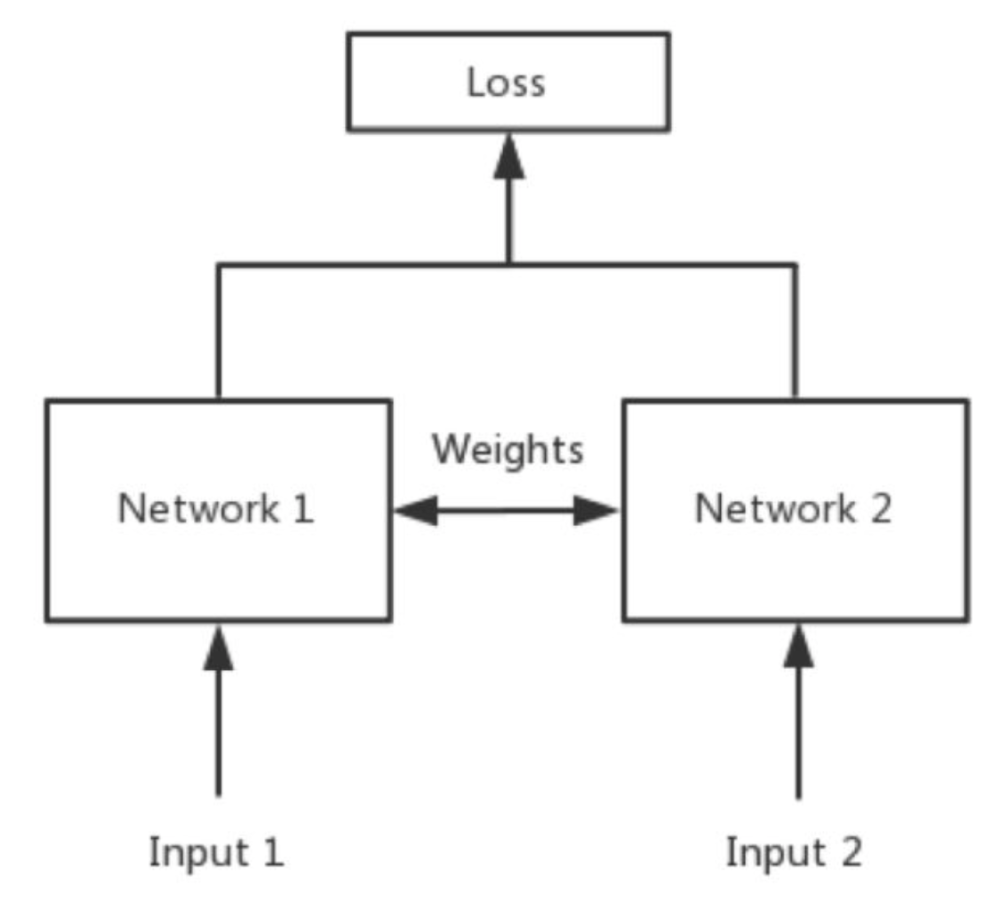
\includegraphics[width=0.7\textwidth]{Siamese network.png}
    \caption{Siamese network}
    \label{fig:Siamese network}
  \end{figure}
\end{enumerate}
\subsubsection{具体实现}
首先,我们划分了训练数据集train\_images和验证数据集val\_images,\\
(见图$\left(\ref{fig:divide1}\right)$)
\begin{figure}[!ht]
  \centering
  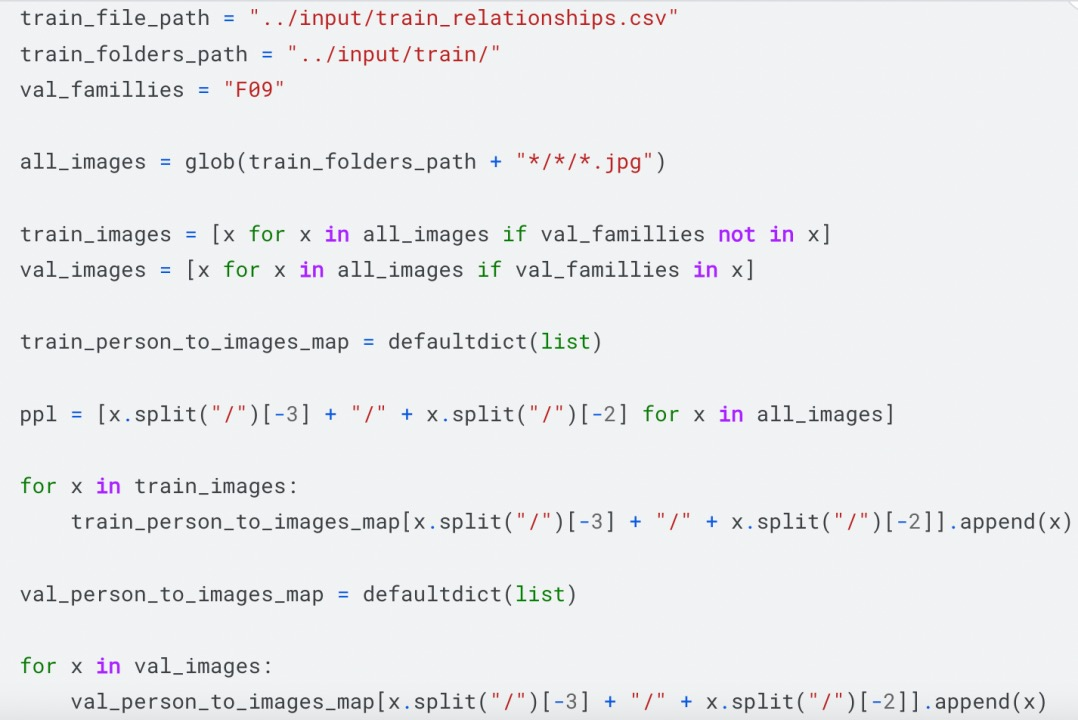
\includegraphics[width=0.5\textwidth]{divide.jpg}
  \label{fig:divide}
\end{figure}
\begin{figure}[!ht]
  \centering
  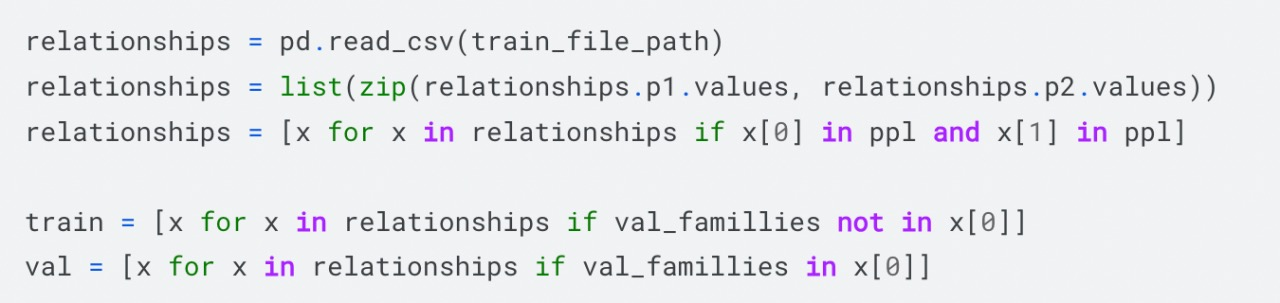
\includegraphics[width=0.5\textwidth]{divide1.jpg}
  \caption{划分训练数据集和验证数据集}
  \label{fig:divide1}
\end{figure}
接下来我们定义一个用于读取图片的函数,该函数需采用已经封装好的preprocess\_input函数。此外,我们还定义了一个生成器,这个生成器的作用是生成训练样本和测试样本。并且要设定相同的正负样本数。通过使用yield语句,能够在迭代的过程当中动态地生成数值。这种方式尤其适用于存在大量数据的情形,它能够助力节省内存空间。

下面载入源自VGG-face数据集预训练的ResNet50模型,进而对模型予以定义。其基本思路为运用若干个Concatante层,之所以如此,是因为并不知晓哪种池化方法更为适宜,也不明确池化后的特征相乘后做差的效果更好,还是做差后相乘的效果更优,故而将这几种处理方式径直进行连接,交由网络自行学习。并采用二元交叉熵充当损失函数。该步骤的具体代码见图$\left(\ref{fig:model}\right)$
\begin{figure}[!ht]
  \centering
  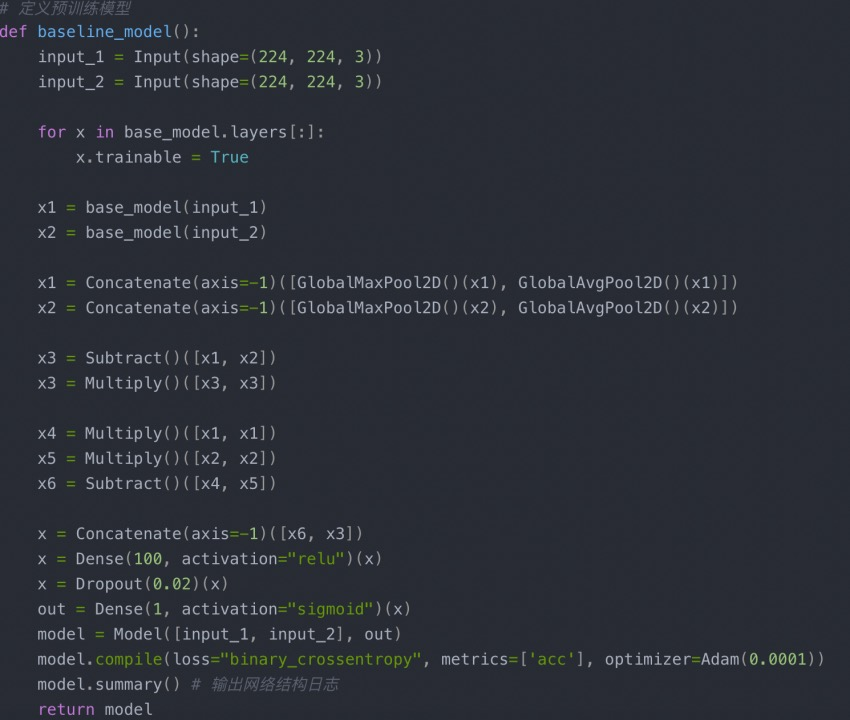
\includegraphics[width=0.7\textwidth]{model.jpg}
  \caption{模型定义}
  \label{fig:model}
\end{figure}

然后我们定义了回调函数,用于保存模型和辅助模型训练,以及进行学习率的设置,代码见图$\left(\ref{fig:func}\right)$
\begin{figure}[!ht]
  \centering
  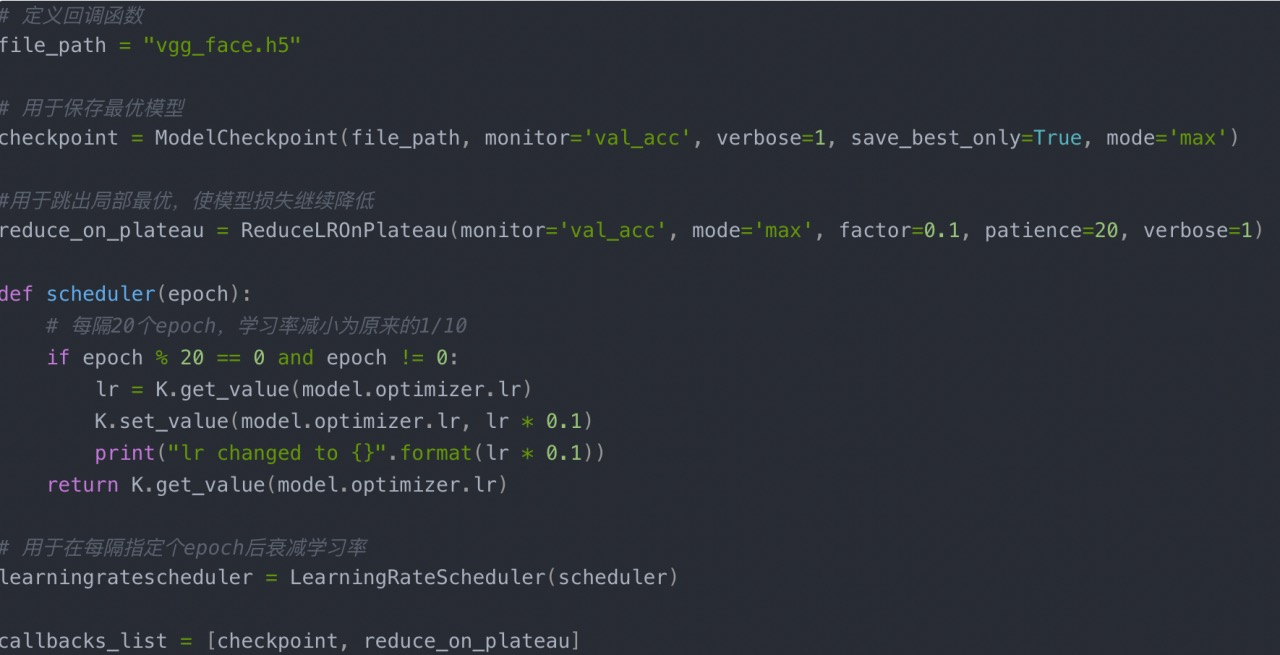
\includegraphics[width=0.7\textwidth]{func.jpg}
  \caption{回调函数}
  \label{fig:func}
\end{figure}

最后实施训练调参操作。首先将mode设置为‘train’,每个epoch迭代200次,总计训练100个epoch。待参数调好之后,再将mode设置为‘train\_valid’,运用全部的数据集重新展开训练,每个epoch迭代300次,同样训练100个epoch。

训练完成后,用该模型对测试集进行预测即可得到输出文件。
\subsection{中期进展结果分析}
在模型训练的过程中我们发现,当不知道怎么处理特征更合适时,可以尝试将不同的特征处理方式串联在一起,交给网络自行去训练,这样可能会得到不错的准确率。

其次,通过使用多个 Concatenate 层,将不同的特征处理方式的结果直接连接在一起,让网络自行学习并权衡各种特征处理方式的重要性。这样的方法可以让模型在训练中学习到更复杂且丰富的特征表示,提高模型的泛化能力。

最后,通过多个 Concatenate 层将不同的特征处理方式连接在一起,可以将不同的处理方式得到的特征融合在一起,这样模型就可以同时考虑多种特征处理方式所得到的特征表示。这种做法旨在让模型自行选择最合适的特征表示方式,从而更好地适应数据。

\subsection{中期进展主要问题分析}
在模型训练的过程中,我们遇到的主要问题是所采用的来自 GitHub 中的 ResNet50 模型所使用的库版本较为陈旧,致使在编译代码时遭遇诸多版本不兼容的问题。除此之外,或许存在效果优于 ResNet50 模型的其他选择,后续我们将会尝试采用其他模型来训练。

\section{中期进展后拟改进措施}
\subsection{特征处理方式}
在处理特征矩阵$x_1$与$x_2$时,我们仅采用了$(x_1-x_2)^2$和$x_1^2-x_2^2$的处理方法,但当我们浏览该比赛的讨论区时,我们发现有的参赛队伍对特征矩阵$x_1$与$x_2$进行了$x_1\times x_2$的操作,后续我们会尝试对特征矩阵进行$x_1\times x_2$的操作,观察模型的得分是否会变高。
\subsection{训练集错误处理}
我们浏览该比赛的讨论区时还发现,官方给出的原始数据中有一些明显错误,如图$\left(\ref{fig:err}\right)$,图片中的两人明显不为同一人,但官方错误将其归类为同一人,这明显导致了我们模型的错误训练。后续我们会尝试直接从官方给出的数据文件夹中删除那些错误的图片,重新训练模型。
\begin{figure}[!ht]
  \centering
  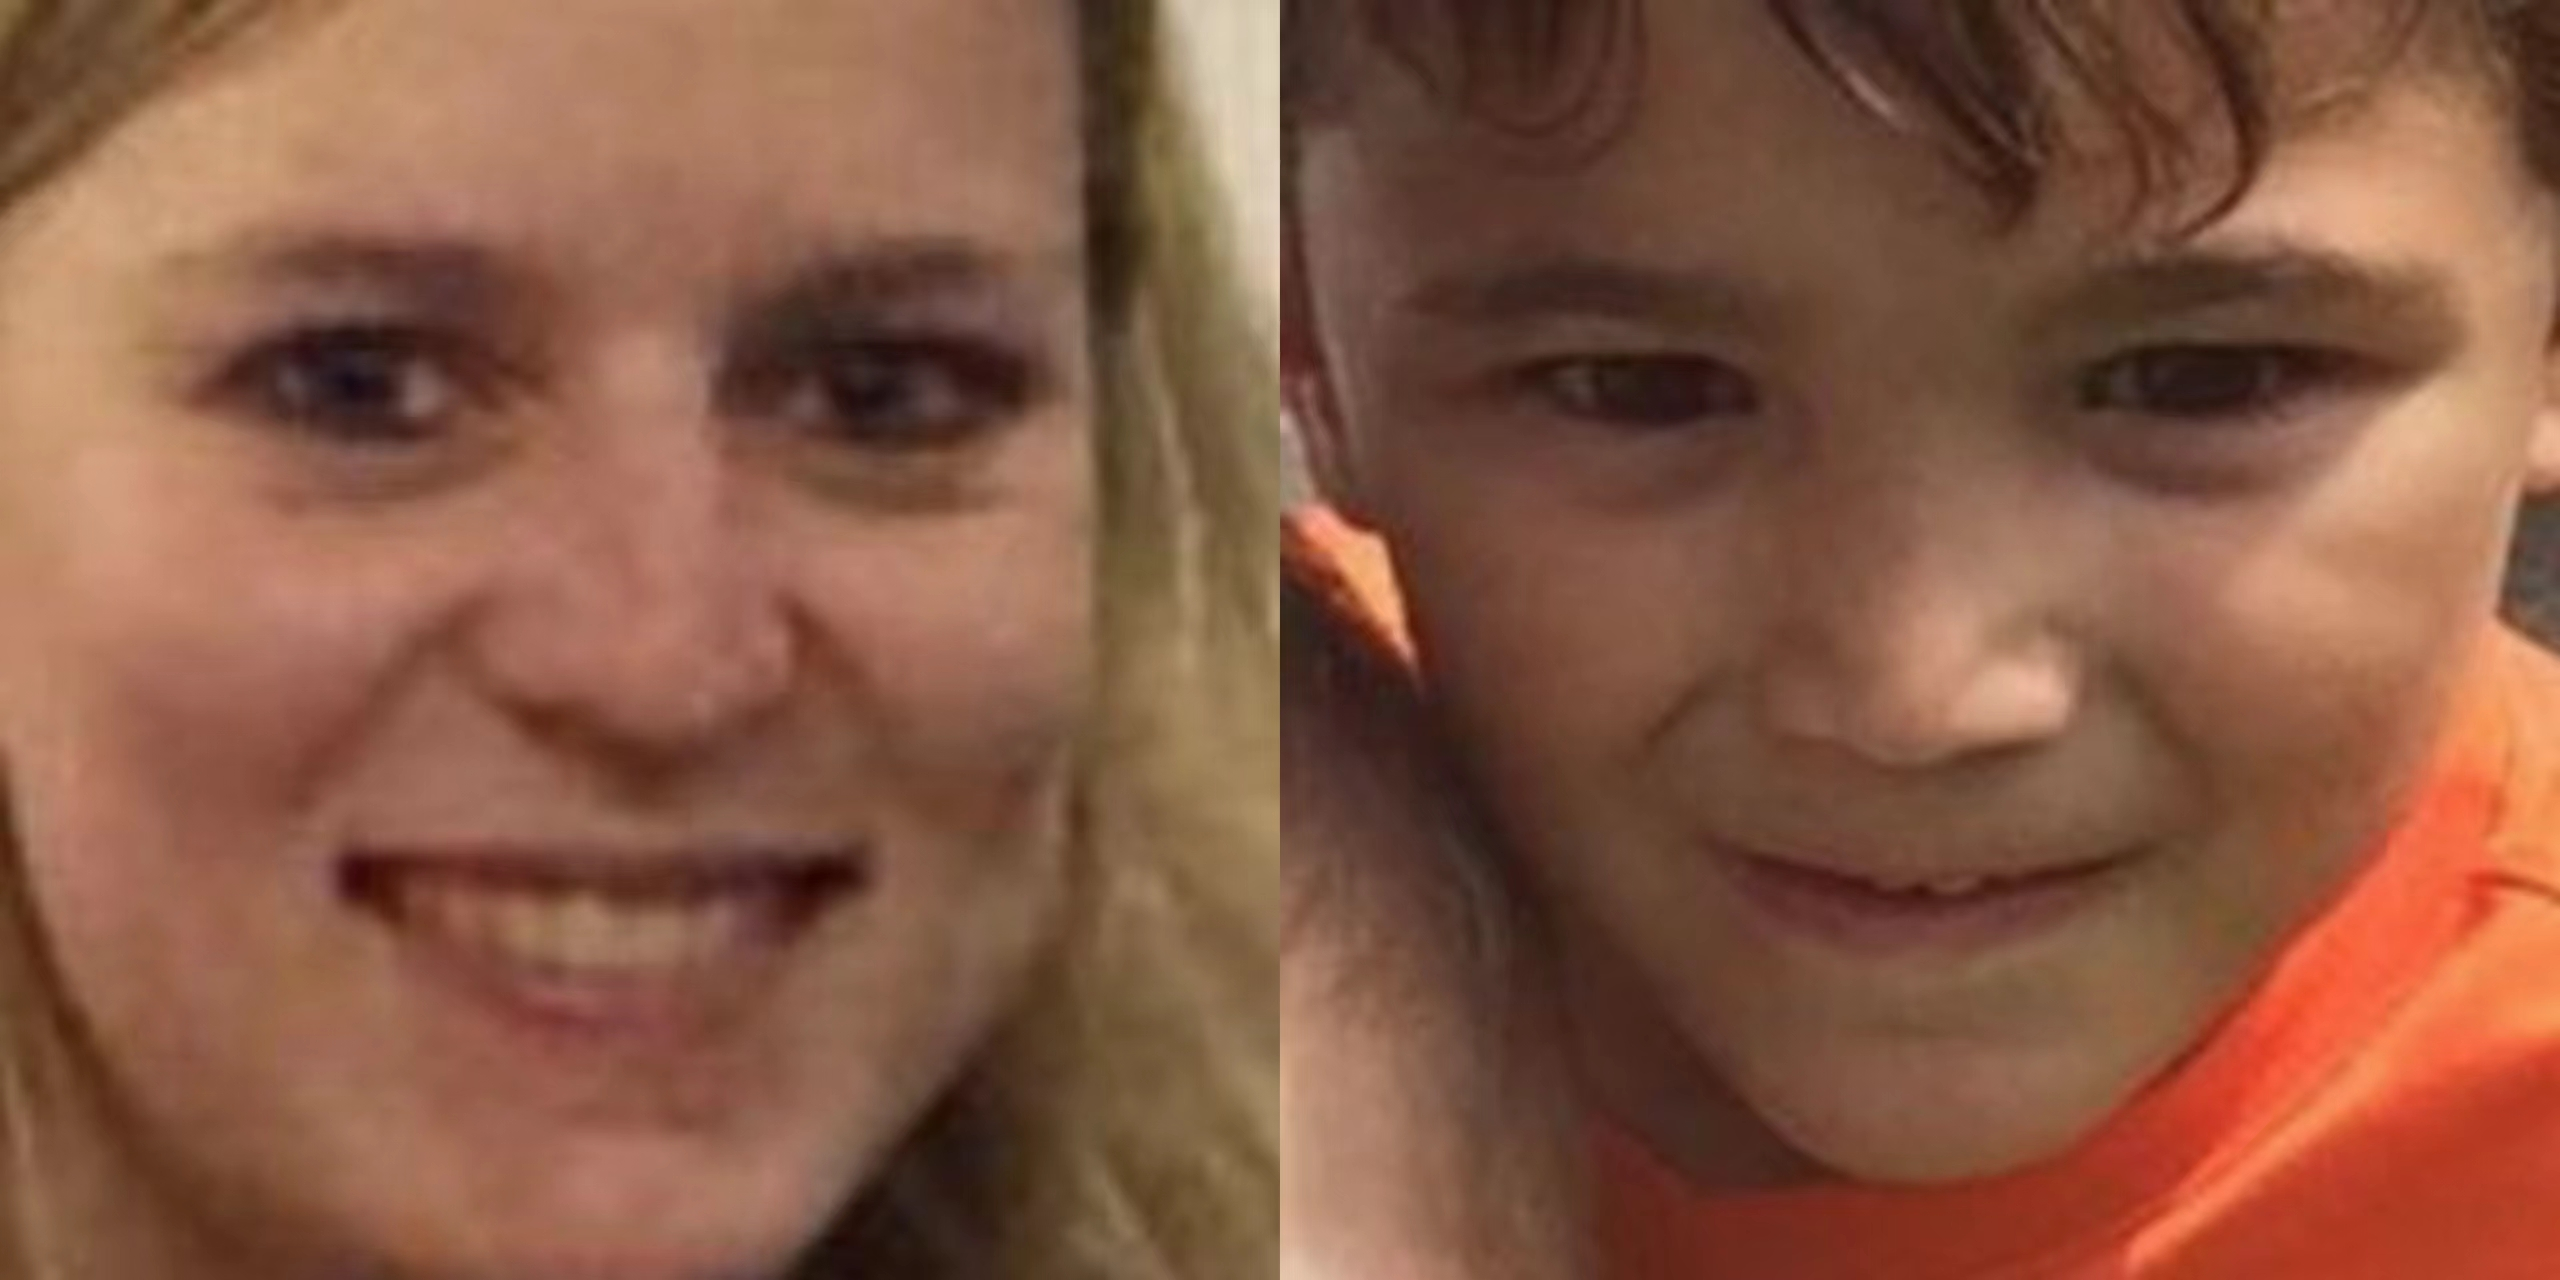
\includegraphics[width=0.7\textwidth]{err.jpg}
  \caption{错误样例1}
  \label{fig:err}
\end{figure}
\subsection{重新选择模型}
经过我们小组成员的讨论,我们决定尝试将ResNet50(Residual Network)模型替换为SENet50(Squeeze-and-Excitation Network)模型。因为SENet引入了一种称为“Squeeze-and-Excitation(SE)”机制的注意力机制,这允许网络学习到每个通道的重要性。使得网络能够更加自适应地关注不同通道之间的关联性,增强特征的表达能力,进而提高网络性能。
\subsection{组合模型}
除此之外,也可以尝试将两个模型组合为一个新的模型。对于每个基于VGGFace的模型x,都有一个基于Facenet的类似模型y。对于这两种模型,得分是相似的,但两个结果几乎无关。作为进一步的步骤,VGGFace和Facenet特征可以在同一模型中组合在一起以生成第三模型z。而第三模型z可能同时具有x与y的优点,这可能对我们提升成绩有所帮助。

\section{参考文献}

\begin{thebibliography}{99}
  \bibitem{1} Koch, G., Zemel, R., \& Salakhutdinov, R. (2015). Siamese Neural Networks for One-shot Image Recognition. In Proceedings of the 32nd International Conference on Machine Learning (ICML) (Vol. 37, pp. 1774-1782).
  \bibitem{2} Song, F., Liu, W., Nie, F., Zhang, W., \& Xu, Z. (2016). Online pair-wise deep hashing with exclusive cross-modal constraints. In Proceedings of the IEEE conference on computer vision and pattern recognition.
  \bibitem{3} He, K., Zhang, X., Ren, S., \& Sun, J. (2016). Deep residual learning for image recognition. In Proceedings of the IEEE conference on computer vision and pattern recognition.
  \bibitem{4} Huang, G., Liu, Z., van der Maaten, L., \& Weinberger, K. Q. (2017). Densely connected convolutional networks. In Proceedings of the IEEE conference on computer vision and pattern recognition.
  \bibitem{5} Zagoruyko, S., \& Komodakis, N. (2015). Learning to compare image patches via convolutional neural networks. In Proceedings of the IEEE conference on computer vision and pattern recognition.
  \bibitem{6} Deng, J., Dong, W., Socher, R., Li, L. J., Li, K., \& Fei-Fei, L. (2009). ImageNet: A large-scale hierarchical image database. In 2009 IEEE conference on computer vision and pattern recognition.
\end{thebibliography}
\end{document}